% document-level settings
\documentclass[border=0.125cm]{standalone}
\usepackage{tikz}
\usepackage{amssymb}
\usepackage{amsmath}
\usepackage{bbm}
\usetikzlibrary{positioning, calc, automata}

\begin{document}

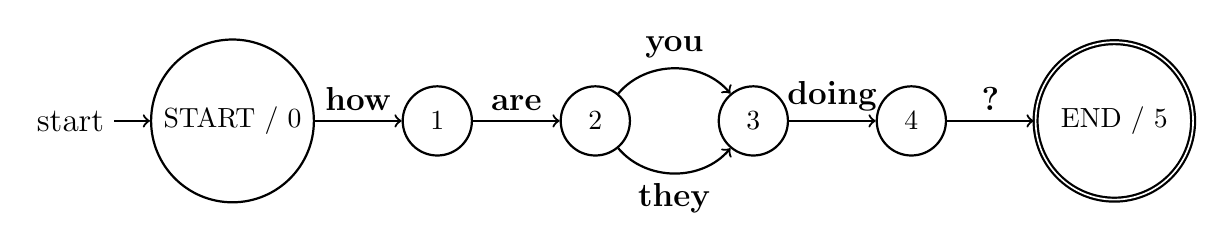
\begin{tikzpicture}[thick, every edge/.append style={font=\large},
  node distance=1.1 cm, every edge/.append style={font=\large}]
  \node[state, initial, minimum size=2cm] (qS_0_0) {START / 0};
  \node[state] (qS_0_1) [right=of qS_0_0] {1}; 
  \node[state] (qS_0_2) [right=of qS_0_1] {2}; 
  \node[state] (qS_0_3) [right=of qS_0_2] {3};
  \node[state] (qS_0_4) [right=of qS_0_3] {4}; 
  \node[state, accepting, minimum size=2cm] (qS_0_5) [right=of qS_0_4] {END / 5}; 
  \path[->] (qS_0_0) edge node[above] {\textbf{how}} (qS_0_1) {};
  \path[->] (qS_0_1) edge node[above] {\textbf{are}} (qS_0_2) {};
  \path[->] (qS_0_2) edge [bend right=50] node [below] {\textbf{they}} (qS_0_3)
  edge [bend left=50]   node [above] {\textbf{you}} (qS_0_3) {};
  \path[->] (qS_0_3) edge node[above] {\textbf{doing}} (qS_0_4) {};
  \path[->] (qS_0_4) edge node[above] {\textbf{?}} (qS_0_5) {};
\end{tikzpicture}

\end{document}